%============================================================
% CHAPITRE IV — Implémentation du firmware générique et intégration
%============================================================
\chapter{Implémentation du firmware générique et intégration}

\section*{Sommaire}
\begin{quote}
\small
\textbf{1} \hspace{1em} Introduction \dotfill \pageref{sec:intro_ch4}\\
\textbf{2} \hspace{1em} Environnement de développement \dotfill \pageref{sec:env_ch4}\\
\hspace{2.5em} 2.1 \hspace{0.5em} ESP-IDF \dotfill \pageref{subsec:espidf}\\
\hspace{2.5em} 2.2 \hspace{0.5em} FreeRTOS \dotfill \pageref{subsec:freertos}\\
\hspace{2.5em} 2.3 \hspace{0.5em} Git et organisation du dépôt \dotfill \pageref{subsec:git}\\
\hspace{2.5em} 2.4 \hspace{0.5em} CI build et conventions de développement \dotfill \pageref{subsec:ci}\\
\hspace{2.5em} 2.5 \hspace{0.5em} Outils de logs, console et debug série \dotfill \pageref{subsec:debug}\\
\textbf{3} \hspace{1em} Mise en place du squelette noyau RTOS \dotfill \pageref{sec:skeleton}\\
\hspace{2.5em} 3.1 \hspace{0.5em} Firmware boot \dotfill \pageref{subsec:boot}\\
\hspace{2.5em} 3.2 \hspace{0.5em} Main task \dotfill \pageref{subsec:maintask}\\
\hspace{2.5em} 3.3 \hspace{0.5em} Event Bus minimal \dotfill \pageref{subsec:evtbus_impl}\\
\hspace{2.5em} 3.4 \hspace{0.5em} Timers système \dotfill \pageref{subsec:timers_impl}\\
\hspace{2.5em} 3.5 \hspace{0.5em} Log série initial \dotfill \pageref{subsec:logserial}\\
\hspace{2.5em} 3.6 \hspace{0.5em} Interface standard des modules \dotfill \pageref{subsec:modiface_impl}\\
\textbf{4} \hspace{1em} Gestion des erreurs et supervision \dotfill \pageref{sec:errors}\\
\hspace{2.5em} 4.1 \hspace{0.5em} Catalogue des codes erreurs \dotfill \pageref{subsec:errcodes}\\
\hspace{2.5em} 4.2 \hspace{0.5em} Niveaux d'erreurs \dotfill \pageref{subsec:errlevels}\\
\hspace{2.5em} 4.3 \hspace{0.5em} Mapping des erreurs \dotfill \pageref{subsec:errmapping}\\
\hspace{2.5em} 4.4 \hspace{0.5em} Watchdog logique noyau \dotfill \pageref{subsec:wdt_impl}\\
\hspace{2.5em} 4.5 \hspace{0.5em} Health counters \dotfill \pageref{subsec:health_impl}\\
\textbf{5} \hspace{1em} Implémentation du module Config \dotfill \pageref{sec:config_impl}\\
\hspace{2.5em} 5.1 \hspace{0.5em} Structure de la configuration persistante \dotfill \pageref{subsec:config_struct}\\
\hspace{2.5em} 5.2 \hspace{0.5em} Gestion version et CRC \dotfill \pageref{subsec:config_crc}\\
\hspace{2.5em} 5.3 \hspace{0.5em} Configuration factory et field \dotfill \pageref{subsec:config_ff}\\
\hspace{2.5em} 5.4 \hspace{0.5em} API config\_get / config\_set / config\_apply \dotfill \pageref{subsec:config_api}\\
\hspace{2.5em} 5.5 \hspace{0.5em} Tests de validation et fallback \dotfill \pageref{subsec:config_tests}\\
\textbf{6} \hspace{1em} Implémentation du module Storage \dotfill \pageref{sec:storage_impl}\\
\hspace{2.5em} 6.1 \hspace{0.5em} Abstraction Storage API \dotfill \pageref{subsec:storage_api}\\
\hspace{2.5em} 6.2 \hspace{0.5em} Définition des partitions log/config/offline \dotfill \pageref{subsec:storage_parts}\\
\hspace{2.5em} 6.3 \hspace{0.5em} Gestion de l'endurance flash \dotfill \pageref{subsec:storage_endur}\\
\hspace{2.5em} 6.4 \hspace{0.5em} Ring buffer simple \dotfill \pageref{subsec:ringbuf}\\
\textbf{7} \hspace{1em} Implémentation du module Logger \dotfill \pageref{sec:logger_impl}\\
\hspace{2.5em} 7.1 \hspace{0.5em} Niveaux de logs \dotfill \pageref{subsec:loglevels}\\
\hspace{2.5em} 7.2 \hspace{0.5em} Logs structurés \dotfill \pageref{subsec:logstruct}\\
\hspace{2.5em} 7.3 \hspace{0.5em} Ring buffer de logs \dotfill \pageref{subsec:logring}\\
\hspace{2.5em} 7.4 \hspace{0.5em} Rotation lorsque le buffer est plein \dotfill \pageref{subsec:logrot}\\
\hspace{2.5em} 7.5 \hspace{0.5em} Dump logs via UART/console \dotfill \pageref{subsec:logdump}\\
\textbf{8} \hspace{1em} Implémentation du Power Manager \dotfill \pageref{sec:power_impl}\\
\hspace{2.5em} 8.1 \hspace{0.5em} Règles RUN/SLEEP \dotfill \pageref{subsec:power_rules}\\
\hspace{2.5em} 8.2 \hspace{0.5em} Sources de réveil : timer et IO \dotfill \pageref{subsec:power_wake}\\
\hspace{2.5em} 8.3 \hspace{0.5em} Réduction de l'activité système \dotfill \pageref{subsec:power_reduce}\\
\hspace{2.5em} 8.4 \hspace{0.5em} Démonstration RUN$\rightarrow$SLEEP et SLEEP$\rightarrow$RUN \dotfill \pageref{subsec:power_demo}\\
\textbf{9} \hspace{1em} Implémentation du Diagnostic \dotfill \pageref{sec:diag_impl}\\
\hspace{2.5em} 9.1 \hspace{0.5em} Reset reason \dotfill \pageref{subsec:diag_reset}\\
\hspace{2.5em} 9.2 \hspace{0.5em} Uptime \dotfill \pageref{subsec:diag_uptime}\\
\hspace{2.5em} 9.3 \hspace{0.5em} Snapshots système \dotfill \pageref{subsec:diag_snap}\\
\hspace{2.5em} 9.4 \hspace{0.5em} État des modules \dotfill \pageref{subsec:diag_mods}\\
\hspace{2.5em} 9.5 \hspace{0.5em} Status report structuré \dotfill \pageref{subsec:diag_report}\\
\textbf{10} \hspace{0.8em} Modularité et intégration \dotfill \pageref{sec:modularite}\\
\hspace{2.5em} 10.1 \hspace{0.5em} HAL v1 \dotfill \pageref{subsec:hal_v1}\\
\hspace{2.5em} 10.2 \hspace{0.5em} Guide d'ajout d'un driver \dotfill \pageref{subsec:hal_guide}\\
\hspace{2.5em} 10.3 \hspace{0.5em} Stubs GNSS et IO \dotfill \pageref{subsec:hal_stubs_impl}\\
\hspace{2.5em} 10.4 \hspace{0.5em} Sélecteur de protocole runtime \dotfill \pageref{subsec:proto_sel}\\
\hspace{2.5em} 10.5 \hspace{0.5em} Intégration avec l'axe configuration/diagnostic \dotfill \pageref{subsec:integ_cfg_diag}\\
\hspace{2.5em} 10.6 \hspace{0.5em} Canal réel USB ou BLE pour config/diag \dotfill \pageref{subsec:canal_reel}\\
\textbf{11} \hspace{0.8em} Gestion des incidents \dotfill \pageref{sec:incidents}\\
\hspace{2.5em} 11.1 \hspace{0.5em} Policies FAULT \dotfill \pageref{subsec:fault_pol}\\
\hspace{2.5em} 11.2 \hspace{0.5em} Backoff \dotfill \pageref{subsec:backoff}\\
\hspace{2.5em} 11.3 \hspace{0.5em} Mode safe \dotfill \pageref{subsec:safemode}\\
\hspace{2.5em} 11.4 \hspace{0.5em} Reprise après reboot \dotfill \pageref{subsec:reboot_resume}\\
\hspace{2.5em} 11.5 \hspace{0.5em} Protection contre les boucles d'erreurs \dotfill \pageref{subsec:antiloop}\\
\textbf{12} \hspace{0.8em} Conclusion \dotfill \pageref{sec:conclu_ch4}\\
\end{quote}

\newpage

%============================================================
\section{Introduction}
\label{sec:intro_ch4}
%============================================================

Ce chapitre présente la mise en œuvre concrète des décisions
architecturales décrites au chapitre précédent. L'objectif est de
traduire chaque choix de conception en code embarqué fonctionnel,
robuste et mesurable, dans le respect des contraintes de ressources
propres aux systèmes industriels déployés sur véhicules. La démarche
adoptée est progressive et itérative : elle débute par la mise en
place de l'environnement de développement et la construction du
squelette multitâche FreeRTOS, socle sur lequel s'appuient tous les
services applicatifs.

Vient ensuite le développement des modules fonctionnels selon leur
ordre de dépendance : le module \texttt{config\_manager} est
implémenté en premier car tous les autres modules dépendent de ses
paramètres, suivi de \texttt{storage\_api}, \texttt{logger},
\texttt{power\_manager} et \texttt{diagnostic}. Les mécanismes de
supervision transverses --- watchdog logiciel à heartbeats, health
counters par module, politique de récupération graduée --- sont
développés en parallèle et intégrés à chaque module dès sa création,
garantissant que la robustesse est une propriété intrinsèque de chaque
composant et non un ajout tardif.

La plateforme cible est l'ESP32-P4, microcontrôleur intégrant deux
cœurs Xtensa LX7 cadencés jusqu'à 400\,MHz, un coprocesseur LP
(\textit{Low Power}) dédié à la surveillance des périphériques en
mode sommeil, ainsi que 8\,Mo de PSRAM et 16\,Mo de Flash intégrés.
Ces capacités matérielles conditionnent directement les choix
d'implémentation décrits dans ce chapitre : la répartition des tâches
sur les deux cœurs exploite le support SMP de FreeRTOS, la stratégie
de partitionnement Flash tire parti des 16\,Mo disponibles pour
héberger deux banques OTA complètes, et le coprocesseur LP est mis
à profit par le \texttt{power\_manager} pour maintenir la surveillance
des sources de réveil à une consommation inférieure à 5\,mA.
L'intégration finale assemble ces composants dans un firmware cohérent,
dont le comportement est validé par des tests unitaires et des mesures
de performance sur cible, présentés au chapitre~V.
%============================================================
\section{Environnement de développement}
\label{sec:env_ch4}
%============================================================

%------------------------------------------------------------
\subsection{Configuration ESP-IDF retenue}
\label{subsec:espidf}
%------------------------------------------------------------

L'ESP-IDF et son rôle de framework de développement ont été présentés
à la section~3.4 du chapitre~II. Dans le cadre du projet
\textit{GlobalFleet}, la version \textbf{v5.3.1 LTS} a été retenue
pour sa stabilité garantie sur 30 mois et sa prise en charge complète
de l'ESP32-P4 avec son c\oe{}ur LP RISC-V.

La configuration spécifique au projet est définie dans le fichier
\texttt{sdkconfig}, versionné dans Git pour garantir la reproductibilité
des builds. Les paramètres critiques sont regroupés en cinq catégories :
schéma de partitionnement Flash via \texttt{partitions.csv}, tailles
des stacks FreeRTOS par tâche, symboles conditionnels
\texttt{CONFIG\_ENABLE\_CAN} et \texttt{CONFIG\_ENABLE\_GNSS} selon
la variante cible, niveaux de log compilés, et paramètres du watchdog
matériel.
\newpage
La toolchain utilisée est \texttt{riscv32-esp-elf-gcc}~13.2.0,
conforme à l'architecture RISC-V de l'ESP32-P4 (voir section~3.1,
chapitre~II). Le pipeline de compilation et de flashage adopté est
illustré à la figure~\ref{fig:build_pipeline}.

\begin{figure}[H]
\centering
\resizebox{\textwidth}{!}{%
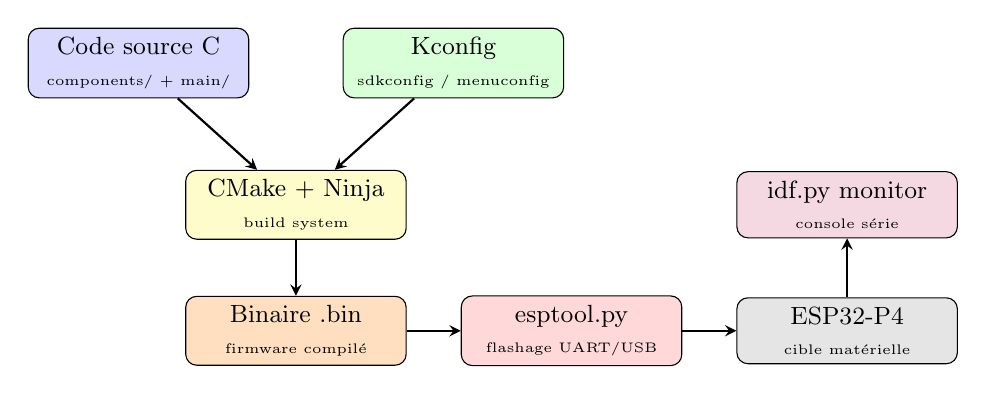
\begin{tikzpicture}[font=\small,
  box/.style={draw, rounded corners=4pt, minimum width=2.8cm,
              minimum height=0.75cm, align=center, fill=#1},
  arr/.style={->, thick, >=stealth}
]
  \node[box=blue!15]   (src)    at (0,0)      {Code source C\\{\tiny components/ + main/}};
  \node[box=green!15]  (kconf)  at (4,0)      {Kconfig\\{\tiny sdkconfig / menuconfig}};
  \node[box=yellow!20] (cmake)  at (2,-1.8)   {CMake + Ninja\\{\tiny build system}};
  \node[box=orange!25] (bin)    at (2,-3.4)   {Binaire .bin\\{\tiny firmware compilé}};
  \node[box=red!15]    (flash)  at (5.5,-3.4) {esptool.py\\{\tiny flashage UART/USB}};
  \node[box=gray!20]   (target) at (9,-3.4)   {ESP32-P4\\{\tiny cible matérielle}};
  \node[box=purple!15] (monitor)at (9,-1.8)   {idf.py monitor\\{\tiny console série}};
  \draw[arr] (src)    -- (cmake);
  \draw[arr] (kconf)  -- (cmake);
  \draw[arr] (cmake)  -- (bin);
  \draw[arr] (bin)    -- (flash);
  \draw[arr] (flash)  -- (target);
  \draw[arr] (target) -- (monitor);
\end{tikzpicture}%
}
\caption{Pipeline de compilation et de flashage ESP-IDF pour le projet
\textit{GlobalFleet} --- toolchain \texttt{riscv32-esp-elf-gcc}~13.2.0}
\label{fig:build_pipeline}
\end{figure}

%------------------------------------------------------------
\subsection{Paramétrage FreeRTOS pour GlobalFleet}
\label{subsec:freertos}
%------------------------------------------------------------

FreeRTOS et son rôle de noyau temps réel ont été présentés et justifiés
à la section~4.1 du chapitre~II. Dans le cadre du projet
\textit{GlobalFleet}, les paramètres FreeRTOS suivants ont été
configurés dans \texttt{sdkconfig} pour répondre aux contraintes
spécifiques du firmware :

\begin{itemize}
  \item Fréquence du tick à \textbf{1000\,Hz} pour une résolution
    temporelle de 1\,ms, permettant des délais précis dans les
    mécanismes de watchdog et de gestion d'énergie.
  \item Taille du heap FreeRTOS à \textbf{256\,Ko}, dimensionné pour
    accueillir les objets de synchronisation (files, mutex, timers)
    de l'ensemble des 23 composants sans risque de saturation.
  \item Activation du support \textbf{SMP} pour l'exploitation des
    deux c\oe{}urs RISC-V HP de l'ESP32-P4, permettant de répartir
    les tâches critiques sur le c\oe{}ur HP0 et les tâches
    applicatives sur le c\oe{}ur HP1 (voir figure~\ref{fig:smp_tasks}).
  \item Activation des \textbf{statistiques de runtime} pour le
    profilage des stacks via \texttt{uxTaskGetStackHighWaterMark()},
    indispensable à la phase de profiling du chapitre~V.
\end{itemize}
\newpage
La répartition des tâches FreeRTOS sur les deux c\oe{}urs de
l'ESP32-P4 est illustrée à la figure~\ref{fig:smp_tasks}. Cette
organisation garantit que les tâches de supervision (watchdog,
dispatcher) ne sont jamais préemptées par les tâches applicatives,
quelle que soit leur charge CPU.

\begin{figure}[H]
\centering
\resizebox{0.85\textwidth}{!}{%
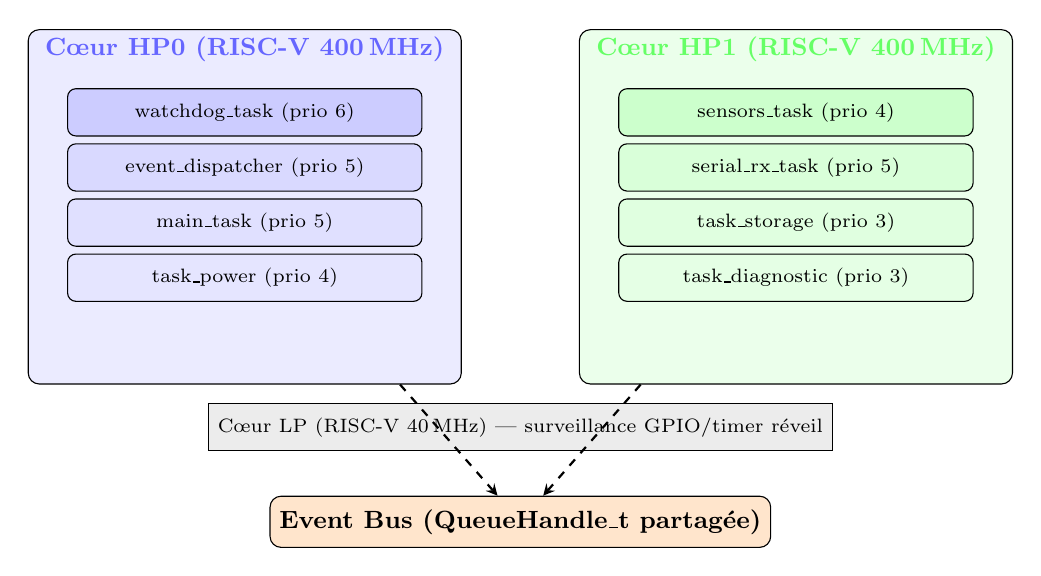
\begin{tikzpicture}[font=\small,
  core/.style={draw, rounded corners=4pt, minimum width=5.5cm,
               minimum height=4.5cm, align=center, fill=#1},
  task/.style={draw, rounded corners=3pt, minimum width=4.5cm,
               minimum height=0.6cm, align=center, fill=#1,
               font=\scriptsize}
]
  \node[core=blue!8] (pro) at (0,0) {};
  \node[font=\bfseries\small, blue!60] at (0, 2.0)
        {C\oe{}ur HP0 (RISC-V 400\,MHz)};
  \node[task=blue!20]   at (0,  1.2) {watchdog\_task (prio 6)};
  \node[task=blue!15]   at (0,  0.5) {event\_dispatcher (prio 5)};
  \node[task=blue!12]   at (0, -0.2) {main\_task (prio 5)};
  \node[task=blue!10]   at (0, -0.9) {task\_power (prio 4)};
  \node[core=green!8] (app) at (7,0) {};
  \node[font=\bfseries\small, green!60] at (7, 2.0)
        {C\oe{}ur HP1 (RISC-V 400\,MHz)};
  \node[task=green!20]  at (7,  1.2) {sensors\_task (prio 4)};
  \node[task=green!15]  at (7,  0.5) {serial\_rx\_task (prio 5)};
  \node[task=green!12]  at (7, -0.2) {task\_storage (prio 3)};
  \node[task=green!10]  at (7, -0.9) {task\_diagnostic (prio 3)};
  \node[draw, fill=gray!15, minimum width=4cm, minimum height=0.6cm,
        align=center, font=\scriptsize] at (3.5,-2.8)
        {C\oe{}ur LP (RISC-V 40\,MHz) --- surveillance GPIO/timer réveil};
  \node[draw, rounded corners=4pt, fill=orange!20, minimum width=5cm,
        minimum height=0.65cm, align=center, font=\bfseries\small]
        (bus) at (3.5,-4.0) {Event Bus (QueueHandle\_t partagée)};
  \draw[->, thick, >=stealth, dashed] (pro) -- (bus);
  \draw[->, thick, >=stealth, dashed] (app) -- (bus);
\end{tikzpicture}%
}
\caption{Répartition SMP des tâches FreeRTOS sur les deux c\oe{}urs RISC-V HP
de l'ESP32-P4 --- paramétrage effectif du projet \textit{GlobalFleet}}
\label{fig:smp_tasks}
\end{figure}

%------------------------------------------------------------
\subsection{Git et organisation du dépôt}
\label{subsec:git}
%------------------------------------------------------------

Le dépôt est organisé selon la convention CMake d'ESP-IDF, adaptée
aux contraintes d'un projet multivariante nécessitant des tests
indépendants par composant. La structure retenue place le point
d'entrée \texttt{app\_main()} et la logique de bootstrap dans le
répertoire \texttt{main/}, les composants fonctionnels dans
\texttt{components/} --- un sous-répertoire par service core, chacun
structuré avec son fichier source \texttt{.c}, son en-tête public
\texttt{.h}, son \texttt{CMakeLists.txt} et potentiellement son
répertoire \texttt{test/} --- les scripts Python et tests Unity
hors-cible dans \texttt{test\_host/}, et la configuration Doxygen
avec la documentation d'architecture dans \texttt{docs/}. La stratégie
de branches Git retenue suit le modèle \textit{Git Flow} : branche
\texttt{main} pour les versions stables, branche \texttt{develop}
pour l'intégration continue, et branches \texttt{feature/xxx} pour
chaque nouveau composant. Les \textit{merge requests} exigent la
validation complète du pipeline CI avant fusion, garantissant qu'aucune
régression de compilation n'est introduite dans la branche principale.

\begin{figure}[H]
\centering
\resizebox{0.80\textwidth}{!}{%
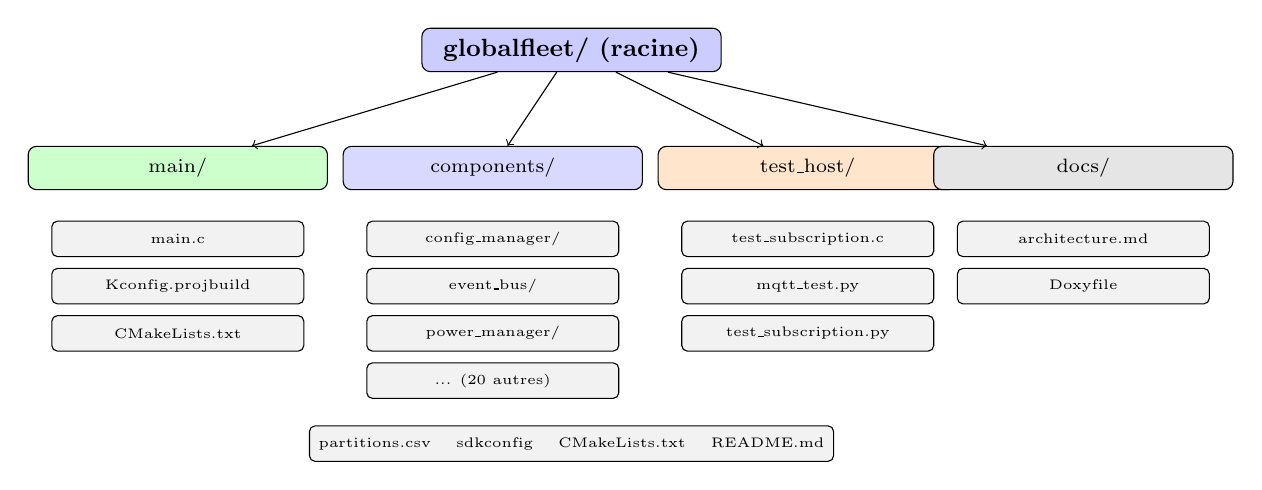
\begin{tikzpicture}[font=\scriptsize,
  folder/.style={draw, rounded corners=3pt, minimum width=3.8cm,
                 minimum height=0.55cm, align=center, fill=#1},
  file/.style={draw, rounded corners=2pt, minimum width=3.2cm,
               minimum height=0.45cm, align=center, fill=gray!10,
               font=\tiny}
]
  \node[folder=blue!20, font=\small\bfseries] (root) at (0,0)
        {globalfleet/ (racine)};
  \node[folder=green!20]  (main)    at (-5,-1.5) {main/};
  \node[folder=blue!15]   (comp)    at (-1,-1.5) {components/};
  \node[folder=orange!20] (thost)   at (3, -1.5) {test\_host/};
  \node[folder=gray!20]   (docs)    at (6.5,-1.5){docs/};
  \draw[->] (root)--(main);
  \draw[->] (root)--(comp);
  \draw[->] (root)--(thost);
  \draw[->] (root)--(docs);
  \node[file] at (-5,-2.4) {main.c};
  \node[file] at (-5,-3.0) {Kconfig.projbuild};
  \node[file] at (-5,-3.6) {CMakeLists.txt};
  \node[file] at (-1,-2.4) {config\_manager/};
  \node[file] at (-1,-3.0) {event\_bus/};
  \node[file] at (-1,-3.6) {power\_manager/};
  \node[file] at (-1,-4.2) {... (20 autres)};
  \node[file] at (3,-2.4) {test\_subscription.c};
  \node[file] at (3,-3.0) {mqtt\_test.py};
  \node[file] at (3,-3.6) {test\_subscription.py};
  \node[file] at (6.5,-2.4) {architecture.md};
  \node[file] at (6.5,-3.0) {Doxyfile};
  \node[file] at (0,-5.0) {partitions.csv \quad sdkconfig \quad CMakeLists.txt \quad README.md};
\end{tikzpicture}%
}
\caption{Structure du dépôt \textit{GlobalFleet} --- organisation CMake/ESP-IDF multivariante}
\label{fig:repo_structure}
\end{figure}
\newpage
%------------------------------------------------------------
\subsection{CI build et conventions de développement}
\label{subsec:ci}
%------------------------------------------------------------

Un pipeline de CI est configuré dès le démarrage du projet pour
garantir la reproductibilité des builds et la détection précoce des
régressions. À chaque \textit{push}, le pipeline exécute quatre
stages en séquence. Le stage \texttt{build} compile le firmware pour
les trois variantes (Basic, Pro, Ultra-Pro) en parallèle, en utilisant
les fichiers \texttt{sdkconfig} de référence versionnés pour chaque
variante. Le stage \texttt{lint} exécute \texttt{clang-tidy}~17.0
avec des règles adaptées au code embarqué C99, vérifiant l'absence
de VLAs, de récursion et d'allocations dynamiques non contrôlées.
Le stage \texttt{size-check} compare les tailles des binaires aux
budgets définis et fait échouer le pipeline si un budget est dépassé,
prévenant la dérive involontaire de la taille du firmware. Le stage
\texttt{artifact} publie les binaires versionnés et le rapport de
taille pour archivage. Les conventions de code appliquées sont les
suivantes : toutes les fonctions publiques sont préfixées par le nom
court du module (\texttt{config\_get()}, \texttt{storage\_write()}),
le type \texttt{esp\_err\_t} est utilisé pour toutes les fonctions
pouvant échouer, et la documentation Doxygen est obligatoire pour
toute API exportée dans un fichier \texttt{.h} public.

%------------------------------------------------------------
\subsection{Outils de logs, console et debug série}
\label{subsec:debug}
%------------------------------------------------------------

Le débogage du firmware repose sur trois outils complémentaires
couvrant les besoins du développement quotidien jusqu'au diagnostic
sur le terrain. Le moniteur série \texttt{idf.py monitor} affiche
les traces UART à 115200 bauds avec coloration syntaxique selon le
niveau de log (\texttt{ESP\_LOGE}, \texttt{ESP\_LOGW}, \texttt{ESP\_LOGI},
\texttt{ESP\_LOGD}), permettant un débogage visuel rapide sans outil
supplémentaire. L'interface JTAG native de l'ESP32-P4 permet
l'exécution pas à pas via GDB et OpenOCD, utile pour les bugs de
concurrence non reproductibles qui ne peuvent être diagnostiqués
uniquement par les traces. Les commandes de diagnostic internes,
accessibles via le canal \texttt{serial\_comm}, exposent à la demande
l'état de chaque module, les watermarks de stack FreeRTOS, l'occupation
heap et les dernières entrées du ring buffer de logs, permettant un
diagnostic complet sur le terrain sans accès à l'infrastructure de
développement.

\begin{table}[H]
\centering
\renewcommand{\arraystretch}{1.5}
\caption{Outils de développement et de débogage du projet \textit{GlobalFleet}}
\label{tab:devtools}
\small
\begin{tabular}{|p{3.0cm}|p{2.5cm}|p{6.0cm}|}
\hline
\rowcolor{gray!20}
\textbf{Outil} & \textbf{Version} & \textbf{Usage principal} \\
\hline
ESP-IDF         & v5.3 LTS    & SDK principal, compilation, flashage, partitionnement \\
\hline
FreeRTOS        & 10.5.1      & RTOS multitâche SMP, files, timers, mutex \\
\hline
CMake / Ninja   & 3.28 / 1.11 & Système de build incrémental multi-variante \\
\hline
clang-tidy      & 17.0        & Analyse statique C99, vérification règles embarquées \\
\hline
Unity           & 2.5.2       & Framework de tests unitaires C hors-cible \\
\hline
OpenOCD / GDB   & 0.12        & Débogage JTAG pas-à-pas sur cible ESP32-P4 \\
\hline
idf.py monitor  & (intégré)   & Console série coloriée + décodage backtrace \\
\hline
esptool.py      & 4.7.0       & Flashage UART/USB et lecture de la Flash \\
\hline
Doxygen         & 1.9.8       & Génération documentation API depuis commentaires \\
\hline
\end{tabular}
\end{table}

%============================================================
\section{Mise en place du squelette noyau RTOS}
\label{sec:skeleton}
%============================================================

Le squelette multitâche constitue le cœur opérationnel du firmware.
Il définit les tâches FreeRTOS, leurs priorités, les mécanismes de
synchronisation inter-tâches et la séquence de démarrage supervisée.
Un squelette bien conçu est la condition sine qua non d'un firmware
robuste : les erreurs d'architecture multitâche sont parmi les plus
difficiles à diagnostiquer en production, car elles se manifestent
de façon non déterministe sous certaines conditions de charge.

%------------------------------------------------------------
\subsection{Firmware boot}
\label{subsec:boot}
%------------------------------------------------------------

La séquence de démarrage du firmware suit cinq étapes ordonnées,
exécutées depuis \texttt{app\_main()} avant la création de toute
tâche applicative. Cette linéarité garantit qu'aucune tâche ne tente
d'accéder à un service non encore initialisé. Premièrement,
l'initialisation du système de fichiers NVS (\texttt{nvs\_flash\_init()})
et la vérification de l'intégrité du schéma de partitionnement.
Deuxièmement, la création et l'initialisation du bus d'événements
via \texttt{event\_bus\_init()}, premier composant instancié car il
ne dépend d'aucun autre service. Troisièmement, le chargement de la
configuration avec vérification CRC par \texttt{config\_manager\_init()}
et activation du fallback si nécessaire. Quatrièmement, la lecture
du registre de capacités et l'instanciation conditionnelle des modules
actifs via la macro \texttt{HAS\_CAPABILITY()}. Cinquièmement, l'appel
séquentiel à \texttt{module\_init()} sur chaque module instancié,
suivi du démarrage du \texttt{watchdog\_task} et de la transition FSM
vers \texttt{RUN} si toutes les initialisations ont réussi. Toute
erreur fatale durant cette séquence publie \texttt{EVT\_FAULT\_CRITICAL}
et provoque la transition vers l'état \texttt{FAULT}.

\begin{figure}[H]
\centering
\resizebox{0.72\textwidth}{!}{%
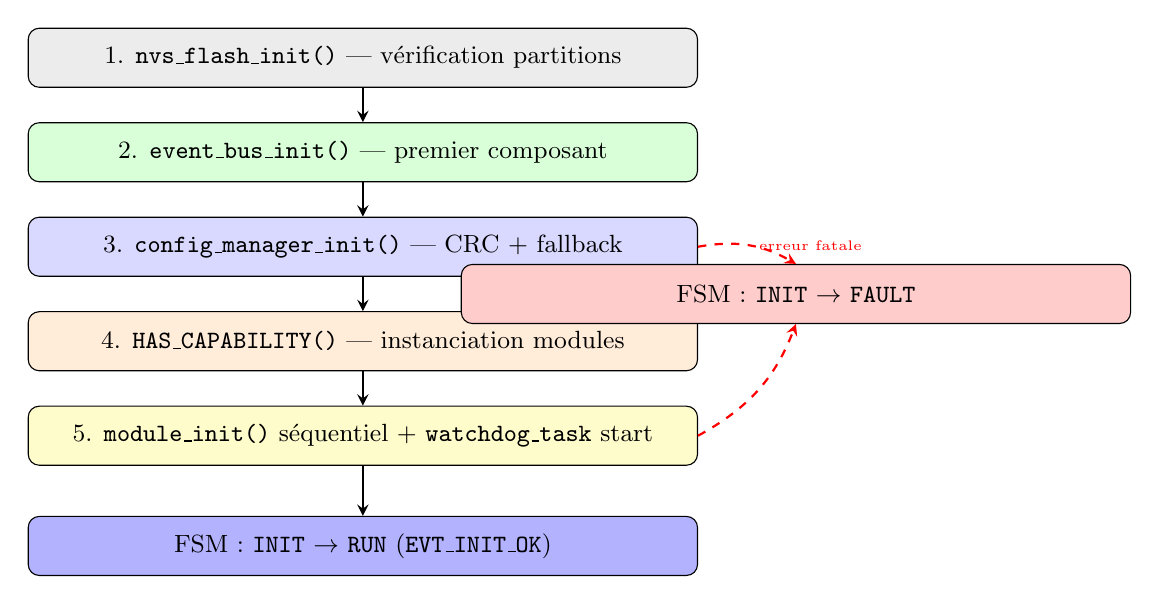
\begin{tikzpicture}[font=\small,
  step/.style={draw, rounded corners=4pt, minimum width=8.5cm,
               minimum height=0.75cm, align=center, fill=#1},
  arrow/.style={->, thick, >=stealth}
]
  \node[step=gray!15]  (s1) at (0, 0)    {1. \texttt{nvs\_flash\_init()} --- vérification partitions};
  \node[step=green!15] (s2) at (0,-1.2)  {2. \texttt{event\_bus\_init()} --- premier composant};
  \node[step=blue!15]  (s3) at (0,-2.4)  {3. \texttt{config\_manager\_init()} --- CRC + fallback};
  \node[step=orange!15](s4) at (0,-3.6)  {4. \texttt{HAS\_CAPABILITY()} --- instanciation modules};
  \node[step=yellow!20](s5) at (0,-4.8)  {5. \texttt{module\_init()} séquentiel + \texttt{watchdog\_task} start};
  \node[step=blue!30]  (s6) at (0,-6.2)  {FSM : \texttt{INIT} $\rightarrow$ \texttt{RUN} (\texttt{EVT\_INIT\_OK})};
  \node[step=red!20]   (sf) at (5.5,-3.0){FSM : \texttt{INIT} $\rightarrow$ \texttt{FAULT}};
  \draw[arrow] (s1)--(s2);
  \draw[arrow] (s2)--(s3);
  \draw[arrow] (s3)--(s4);
  \draw[arrow] (s4)--(s5);
  \draw[arrow] (s5)--(s6);
  \draw[->, thick, >=stealth, red, dashed]
        (s3.east) to[bend left=20]
        node[right, font=\tiny, red]{erreur fatale} (sf.north);
  \draw[->, thick, >=stealth, red, dashed]
        (s5.east) to[bend right=20] (sf.south);
\end{tikzpicture}%
}
\caption{Séquence de boot du firmware \textit{GlobalFleet} --- 5 étapes ordonnées depuis \texttt{app\_main()}}
\label{fig:boot_seq}
\end{figure}

\begin{figure}[H]
  \centering
  
\includegraphics[width=0.60\textwidth]{figures/esp32p4_chip.png}
  \caption{Microcontrôleur ESP32-P4 --- plateforme cible du firmware \textit{GlobalFleet}
           (dual-core Xtensa LX7, coprocesseur LP, 16\,Mo Flash, 8\,Mo PSRAM)}
  \label{fig:esp32p4}
\end{figure}

%------------------------------------------------------------
\subsection{Main task}
\label{subsec:maintask}
%------------------------------------------------------------

La \textit{main task}, nommée \texttt{task\_supervisor}, est la tâche
FreeRTOS de priorité la plus élevée du système (priorité~10). Elle
remplit trois responsabilités après le boot : piloter la FSM système
en réaction aux événements de transition reçus via le bus d'événements,
alimenter le watchdog logiciel noyau en émettant ses propres heartbeats
périodiques, et surveiller l'état de santé global du système via les
health counters des modules. Sa haute priorité garantit qu'elle est
préemptée uniquement par les interruptions matérielles et le timer
FreeRTOS, lui permettant de réagir aux événements critiques même
lorsque les tâches applicatives sont sous forte charge. Elle est
affinée sur le cœur PRO (CPU0) pour isoler son exécution des tâches
applicatives réparties sur le cœur APP (CPU1). Le tableau~\ref{tab:tasks}
récapitule l'ensemble des neuf tâches créées dans le squelette, avec
leurs priorités, tailles de stack et affinités de cœur.

\begin{table}[H]
\centering
\renewcommand{\arraystretch}{1.6}
\caption{Hiérarchie des tâches FreeRTOS du firmware \textit{GlobalFleet}}
\label{tab:tasks}
\small
\begin{tabular}{|p{3.8cm}|c|c|c|p{3.2cm}|}
\hline
\rowcolor{gray!20}
\textbf{Tâche} & \textbf{Prio.} & \textbf{Stack} & \textbf{Cœur} & \textbf{Rôle} \\
\hline
\texttt{task\_supervisor}        & 10 & 4096\,o & PRO & FSM + watchdog noyau \\
\hline
\texttt{task\_event\_dispatcher} & 8  & 4096\,o & PRO & Distribution Event Bus \\
\hline
\texttt{task\_gnss}              & 7  & 4096\,o & APP & Parsing NMEA / UBX \\
\hline
\texttt{task\_can}               & 7  & 4096\,o & APP & Lecture bus CAN J1939 \\
\hline
\texttt{task\_comms}             & 6  & 6144\,o & PRO & MQTT/TLS + reconnexion \\
\hline
\texttt{task\_storage}           & 5  & 4096\,o & APP & Écriture Flash + logs \\
\hline
\texttt{task\_power}             & 5  & 3072\,o & PRO & Transitions énergie \\
\hline
\texttt{task\_diagnostic}        & 4  & 4096\,o & APP & Métriques + snapshots \\
\hline
\texttt{task\_config}            & 3  & 3072\,o & APP & Commandes config série \\
\hline
\end{tabular}
\end{table}

%------------------------------------------------------------
\subsection{Event Bus minimal}
\label{subsec:evtbus_impl}
%------------------------------------------------------------

L'Event Bus est le premier composant initialisé car il ne dépend
d'aucun autre service du firmware. Son implémentation dans le composant
\texttt{event\_bus} repose sur une file FreeRTOS
\texttt{QueueHandle\_t} de capacité configurable via
\texttt{CONFIG\_EVENT\_BUS\_QUEUE\_SIZE} (32 événements par défaut),
et une table de souscription statique associant chaque type d'événement
à une liste de callbacks enregistrés par les modules lors de leur
initialisation. La fonction \texttt{event\_bus\_post()} est
thread-safe et ISR-safe : elle utilise \texttt{xQueueSend()} en
contexte de tâche normale et \texttt{xQueueSendFromISR()} depuis
un handler d'interruption, permettant aux drivers HAL de publier
des événements depuis le contexte d'interruption sans risque de
blocage. La tâche \texttt{task\_event\_dispatcher} lit la file en
mode bloquant (attente infinie) et appelle séquentiellement tous
les callbacks abonnés à chaque type d'événement reçu. Cette
architecture garantit que les callbacks sont toujours exécutés
dans le contexte de la tâche dispatcher, protégeant les modules
consommateurs des problèmes de concurrence avec les producteurs
ISR.

%------------------------------------------------------------
\subsection{Timers système}
\label{subsec:timers_impl}
%------------------------------------------------------------

Quatre timers logiciels FreeRTOS (\texttt{TimerHandle\_t}) sont
instanciés dans le noyau lors de la phase d'initialisation. Le timer
de rapport périodique déclenche l'envoi d'un statut vers le serveur
à la période \texttt{cfg.comms.report\_interval\_s}. Le timer
watchdog vérifie à intervalle régulier que chaque module enregistré
a émis son heartbeat dans la fenêtre \texttt{cfg.kernel.wdt\_timeout\_ms}.
Le timer de rotation des logs déclenche la purge du ring buffer RAM
vers la Flash à intervalle configurable, garantissant que les logs
sont persistés même en l'absence d'événements déclencheurs. Le timer
anti-boucle maintient et décrémente le compteur de redémarrages dans
une fenêtre glissante de 60~secondes. Toutes les périodes sont lues
depuis la configuration terrain au démarrage via \texttt{config\_manager}
et reconfigurées dynamiquement à la réception de l'événement
\texttt{EVT\_CONFIG\_CHANGED}, permettant d'ajuster les intervalles
sans redémarrer le système.

%------------------------------------------------------------
\subsection{Log série initial}
\label{subsec:logserial}
%------------------------------------------------------------

Avant l'initialisation complète du module \texttt{logger}, les
premières traces de démarrage sont émises directement via les macros
\texttt{ESP\_LOGx()} d'ESP-IDF sur le port UART0 (115200~bauds,
8N1). Chaque entrée inclut un horodatage relatif en millisecondes
depuis le boot, le niveau de sévérité colorisé (\texttt{E}, \texttt{W},
\texttt{I}, \texttt{D}), et le tag du composant émetteur sur 12
caractères maximum. Ce canal de log brut reste actif pendant toute
la durée de vie du firmware comme filet de sécurité indépendant de
l'état du module \texttt{logger} : même en cas de défaillance du
module Logger ou de corruption de la partition \texttt{logs}, les
traces de boot critiques restent accessibles via le canal UART0,
permettant le diagnostic des défaillances au premier démarrage.

%------------------------------------------------------------
\subsection{Interface standard des modules}
\label{subsec:modiface_impl}
%------------------------------------------------------------

Tous les composants du firmware implémentent la structure
\texttt{module\_interface\_t} définie dans
\texttt{components/module\_interface/include/module\_interface.h}.
Cette structure de pointeurs de fonctions impose quatre points d'entrée
obligatoires et deux champs d'état permettant la supervision uniforme
par le noyau. La fonction \texttt{init()} initialise les ressources
internes et enregistre les abonnements au bus. La fonction
\texttt{start()} crée la tâche FreeRTOS associée via
\texttt{xTaskCreatePinnedToCore()}, en spécifiant la taille de stack
et la priorité dimensionnées dans les constantes du composant. La
fonction \texttt{stop()} arrête proprement la tâche et libère les
ressources, garantissant l'absence de fuite lors des redémarrages
partiels gérés par le \texttt{fault\_manager}. La fonction
\texttt{handle\_event(event*)} est le callback du dispatcher. Les
champs \texttt{state} (\texttt{IDLE}/\texttt{RUNNING}/\texttt{FAULT})
et \texttt{health\_counter} sont maintenus par le module lui-même
et consultés par le \texttt{diagnostic}. La fonction \texttt{app\_main()}
boucle sur la liste des modules instanciés, appelle \texttt{init()}
sur chacun, puis \texttt{start()} si toutes les initialisations ont
réussi.

%============================================================
\section{Gestion des erreurs et supervision}
\label{sec:errors}
%============================================================

La gestion des erreurs est une préoccupation transverse qui concerne
l'ensemble des modules du firmware. Une architecture d'erreur bien
conçue garantit que toute défaillance, quelle que soit son origine,
est détectée, classifiée et traitée de manière cohérente, sans créer
de comportements indéfinis ni de blocages du système. Cette section
décrit les mécanismes implémentés dans les composants
\texttt{error\_manager}, \texttt{watchdog\_task} et
\texttt{module\_health}.

%------------------------------------------------------------
\subsection{Catalogue des codes erreurs}
\label{subsec:errcodes}
%------------------------------------------------------------

Un catalogue centralisé de codes d'erreurs est défini dans
\texttt{components/error\_manager/include/error\_codes.h}. Chaque
code est un entier 32~bits organisé en trois champs selon une structure
de bits dédiée : les bits 31--24 identifient le module émetteur
(8~bits, 256 modules maximum), les bits 23--16 encodent le type de
l'erreur (8~bits, 256 types), et les bits 15--0 contiennent le code
détaillé (16~bits, 65536 codes par type). Cette structure permet de
filtrer les erreurs par module ou par type avec de simples opérations
de masquage binaire (\texttt{err \& MODULE\_MASK}), facilitant le
diagnostic et le routage des erreurs vers les handlers appropriés.
Le catalogue couvre quatre domaines fonctionnels principaux : les
erreurs de configuration (préfixe \texttt{ERR\_CFG\_}), de stockage
(\texttt{ERR\_STG\_}), de communication (\texttt{ERR\_COMMS\_}) et
de supervision noyau (\texttt{ERR\_WDT\_}, \texttt{ERR\_DIAG\_}).

\begin{table}[H]
\centering
\renewcommand{\arraystretch}{1.5}
\caption{Extrait du catalogue des codes d'erreurs système --- \texttt{error\_codes.h}}
\label{tab:errcodes}
\small
\begin{tabular}{|l|p{2.2cm}|p{5.5cm}|}
\hline
\rowcolor{gray!20}
\textbf{Code} & \textbf{Module} & \textbf{Description} \\
\hline
\texttt{ERR\_CFG\_CRC\_INVALID}    & config\_manager & CRC-32 de la configuration invalide \\
\hline
\texttt{ERR\_CFG\_VER\_MISMATCH}   & config\_manager & Version incompatible avec le firmware \\
\hline
\texttt{ERR\_STG\_PARTITION\_FULL} & storage\_api    & Partition offline saturée ($>$seuil) \\
\hline
\texttt{ERR\_STG\_WRITE\_FAIL}     & storage\_api    & Échec d'écriture Flash (secteur défaillant) \\
\hline
\texttt{ERR\_PWR\_WAKE\_TIMEOUT}   & power\_manager  & Réveil sans source identifiée \\
\hline
\texttt{ERR\_WDT\_TASK\_TIMEOUT}   & watchdog\_task  & Heartbeat manquant d'une tâche enregistrée \\
\hline
\texttt{ERR\_COMMS\_CONN\_LOST}    & comms\_manager  & Perte de connectivité réseau \\
\hline
\texttt{ERR\_DIAG\_NVS\_FULL}      & diagnostic      & Partition diag NVS saturée \\
\hline
\end{tabular}
\end{table}

%------------------------------------------------------------
\subsection{Niveaux d'erreurs}
\label{subsec:errlevels}
%------------------------------------------------------------

Quatre niveaux de sévérité sont définis dans \texttt{error\_manager},
en cohérence directe avec la politique de récupération de la FSM.
Le niveau \textbf{WARNING} signale une dégradation non critique :
le système continue sans interruption, le compteur de santé du module
est incrémenté de un, et une entrée est ajoutée au \texttt{logger}.
Le niveau \textbf{ERROR} indique la défaillance d'un composant non
critique : le module fautif est redémarré par le \texttt{fault\_manager}
avec un délai selon la stratégie de backoff exponentiel. Le niveau
\textbf{CRITICAL} désigne une défaillance affectant la sûreté du
système : un redémarrage complet est déclenché en publiant
\texttt{EVT\_FAULT\_CRITICAL} sur le bus. Le niveau \textbf{FATAL}
est atteint après plusieurs tentatives de récupération infructueuses
détectées par le mécanisme anti-boucle : le mode safe minimal est
activé, suspendant tous les modules non essentiels et transmettant
un rapport de diagnostic au serveur.

%------------------------------------------------------------
\subsection{Mapping des erreurs}
\label{subsec:errmapping}
%------------------------------------------------------------

Le mapping traduit les codes d'erreur ESP-IDF (\texttt{esp\_err\_t})
vers les codes internes du firmware. Cette couche de traduction est
définie dans une table statique dans \texttt{error\_manager.c} et
consultée à chaque appel à \texttt{error\_report()}. Elle isole
totalement le code applicatif des valeurs ESP-IDF spécifiques à la
plateforme, ce qui présente deux avantages. Premièrement, le code
applicatif ne dépend pas des valeurs numériques ESP-IDF qui pourraient
changer d'une version d'ESP-IDF à l'autre. Deuxièmement, les tests
unitaires hors-cible dans \texttt{test\_host/} peuvent substituer
les retours ESP-IDF par des valeurs simulées sans modifier le code
testé, facilitant l'injection de conditions d'erreur dans les
scénarios de test de robustesse.

%------------------------------------------------------------
\subsection{Watchdog logique noyau}
\label{subsec:wdt_impl}
%------------------------------------------------------------

Le composant \texttt{watchdog\_task} implémente un watchdog logiciel
multi-tâches distinct du watchdog matériel ESP-IDF, conçu pour détecter
les blocages applicatifs de niveau tâche que le watchdog matériel ne
peut pas distinguer d'un fonctionnement normal. Chaque module
actif s'enregistre auprès du watchdog lors de son initialisation via
\texttt{wdt\_register(module\_id, timeout\_ms)} et doit ensuite
appeler périodiquement \texttt{wdt\_kick(module\_id)} depuis sa
tâche principale. Le timer watchdog vérifie toutes les
\texttt{cfg.kernel.wdt\_check\_period\_ms} millisecondes que chaque
module enregistré a émis son heartbeat dans la fenêtre configurée.
En l'absence de heartbeat --- indiquant un blocage sur une ressource,
une boucle infinie, ou un crash silencieux --- l'erreur
\texttt{ERR\_WDT\_TASK\_TIMEOUT} est remontée au \texttt{error\_manager}
avec le niveau CRITICAL, et l'événement \texttt{EVT\_WDT\_TIMEOUT}
est publié sur le bus avec en payload l'identifiant de la tâche
défaillante, déclenchant la politique de récupération du
\texttt{fault\_manager}.

\begin{figure}[H]
\centering
\resizebox{0.85\textwidth}{!}{%
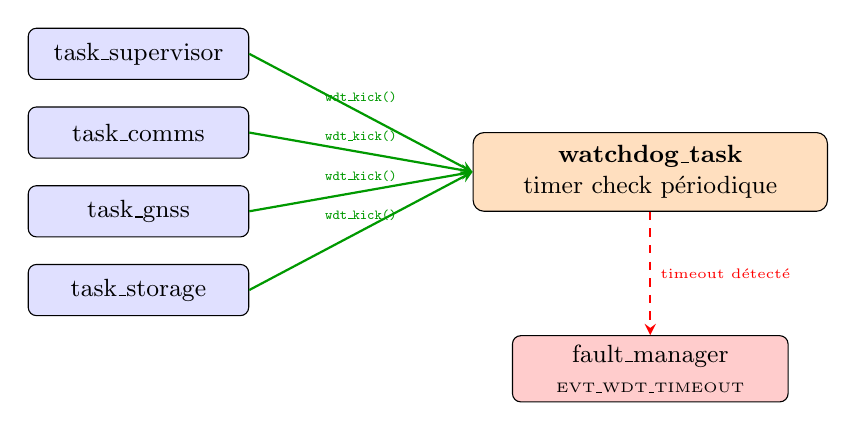
\begin{tikzpicture}[font=\small,
  mod/.style={draw, rounded corners=3pt, minimum width=2.8cm,
              minimum height=0.65cm, align=center, fill=blue!12},
  wdt/.style={draw, rounded corners=4pt, minimum width=4.5cm,
              minimum height=1.0cm, align=center, fill=orange!25,
              font=\bfseries\small},
  arr/.style={->, thick, >=stealth}
]
  \node[wdt] (wdt) at (6.5, 0) {watchdog\_task\\{\small\normalfont timer check périodique}};
  \node[mod] (m1) at (0, 1.5)  {task\_supervisor};
  \node[mod] (m2) at (0, 0.5)  {task\_comms};
  \node[mod] (m3) at (0,-0.5)  {task\_gnss};
  \node[mod] (m4) at (0,-1.5)  {task\_storage};
  \foreach \m in {m1,m2,m3,m4}
    \draw[arr, green!60!black] (\m.east) -- node[above, font=\tiny]{\texttt{wdt\_kick()}} (wdt.west);
  \node[draw, rounded corners=3pt, fill=red!20, minimum width=3.5cm,
        minimum height=0.65cm, align=center]
        (fault) at (6.5,-2.5) {fault\_manager\\{\tiny EVT\_WDT\_TIMEOUT}};
  \draw[arr, red, dashed, thick] (wdt) -- node[right, font=\tiny]{timeout détecté} (fault);
\end{tikzpicture}%
}
\caption{Mécanisme de watchdog logiciel multi-tâches --- composant \texttt{watchdog\_task}}
\label{fig:wdt_mechanism}
\end{figure}

%------------------------------------------------------------
\subsection{Health counters}
\label{subsec:health_impl}
%------------------------------------------------------------

Des compteurs de santé sont maintenus pour chaque module dans le
champ \texttt{health\_counter} de la structure
\texttt{module\_interface\_t}. Le compteur est incrémenté de~1 à
chaque anomalie non critique signalée par le module (timeout de file
d'attente, erreur driver transitoire, valeur hors plage) et décrémenté
de~1 toutes les \texttt{HEALTH\_DECAY\_PERIOD\_MS} millisecondes par
un timer dédié dans le \texttt{module\_health}. Ce mécanisme de
décroissance temporelle permet de distinguer les erreurs ponctuelles
--- dont le compteur revient rapidement à zéro sans atteindre de seuil
--- des dégradations persistantes, dont le compteur croît jusqu'au
seuil d'alerte. Trois seuils configurables sont définis :
\texttt{HEALTH\_WARN\_THRESHOLD} déclenche une journalisation sans
action, \texttt{HEALTH\_ERROR\_THRESHOLD} déclenche un redémarrage
du module via l'interface \texttt{module\_stop()} / \texttt{module\_start()}
avec backoff exponentiel, et \texttt{HEALTH\_CRITICAL\_THRESHOLD}
déclenche un redémarrage système complet en publiant
\texttt{EVT\_FAULT\_CRITICAL}. Ce mécanisme graduel évite les
redémarrages intempestifs liés à des erreurs transitoires tout en
garantissant la détection des dégradations progressives avant qu'elles
ne deviennent critiques pour la continuité de service.

%============================================================
\section{Implémentation du module Config}
\label{sec:config_impl}
%============================================================

%------------------------------------------------------------
\subsection{Structure de la configuration persistante}
\label{subsec:config_struct}
%------------------------------------------------------------

La configuration persistante est organisée en une structure C plate
(\textit{flat struct}) de taille fixe, sérialisée en binaire dans
la partition NVS. L'utilisation d'une taille fixe est délibérée :
elle garantit que le CRC-32 couvre toujours l'intégralité des champs
sans calcul de longueur dynamique, évitant les bugs subtils de
validation partielle qui pourraient laisser passer une configuration
corrompue. La structure est subdivisée en sous-structures par domaine
fonctionnel pour faciliter la lisibilité et les tests par composant :
\texttt{cfg\_header\_t} (version, CRC), \texttt{cfg\_network\_t}
(APN, serveur, port), \texttt{cfg\_comms\_t} (protocole, QoS, topics
MQTT), \texttt{cfg\_power\_t} (paramètres de veille, sources de
réveil) et \texttt{cfg\_thresholds\_t} (seuils de détection, intervalles
de rapport). La structure complète est définie dans
\texttt{components/config\_manager/include/config\_types.h} et
exportée comme type opaque aux autres composants, qui n'accèdent
aux champs que via l'API \texttt{config\_get()} / \texttt{config\_set()}.

%------------------------------------------------------------
\subsection{Gestion version et CRC}
\label{subsec:config_crc}
%------------------------------------------------------------

Le premier champ de la structure est un en-tête \texttt{cfg\_header\_t}
contenant le numéro de version sur 16~bits et le CRC-32 calculé sur
tous les champs suivants (en excluant l'en-tête lui-même, pour éviter
la circularité). Au chargement depuis la partition \texttt{nvs\_field},
le module \texttt{config\_manager} exécute trois vérifications
successives. Premièrement, il calcule le CRC-32 de la structure lue
depuis NVS et compare le résultat au champ \texttt{header.crc32}
persisté. Deuxièmement, si le CRC est valide, il compare le numéro
de version au numéro attendu par le firmware courant, compilé en dur
dans la constante \texttt{CONFIG\_EXPECTED\_VERSION}. Troisièmement,
si les deux vérifications réussissent, la configuration est chargée
en mémoire cache et considérée valide. En cas d'échec de l'une ou
l'autre vérification, le fallback factory est déclenché, un événement
\texttt{EVT\_CONFIG\_CHANGED} est publié avec le flag
\texttt{is\_fallback = true}, et une entrée WARNING est ajoutée
au \texttt{logger}.

%------------------------------------------------------------
\subsection{Configuration factory et field}
\label{subsec:config_ff}
%------------------------------------------------------------

La configuration factory est lue depuis la partition NVS
\texttt{nvs\_factory} au démarrage et mise en cache en mémoire RAM
pour les accès ultérieurs sans I/O NVS. Elle contient les paramètres
immuables programmés en usine : numéro de série, type de matériel,
registre de capacités initial, clés TLS de l'appareil, et adresse
du serveur de référence. Le drapeau \texttt{factory\_locked} persisté
dans cette partition empêche toute écriture depuis le code applicatif :
toute tentative de modification d'une clé factory via
\texttt{config\_set()} est immédiatement rejetée avec le code
d'erreur \texttt{ERR\_CFG\_FACTORY\_LOCKED}. La configuration field
est lue et écrite depuis la partition \texttt{nvs\_field}. Elle
contient les paramètres opérationnels modifiables à distance.
Une mise à jour field passe obligatoirement par \texttt{config\_apply()},
qui valide les plages de valeurs, calcule le nouveau CRC-32, et
persiste atomiquement avant de publier \texttt{EVT\_CONFIG\_CHANGED}.

%------------------------------------------------------------
\subsection{API config\_get / config\_set / config\_apply}
\label{subsec:config_api}
%------------------------------------------------------------

L'interface publique du module \texttt{config\_manager} expose trois
fonctions principales formant un mécanisme transactionnel de modification
de configuration. \texttt{config\_get(key, buf, len)} retourne la
valeur courante d'un paramètre identifié par sa clé textuelle, depuis
le cache mémoire sans I/O NVS. \texttt{config\_set(key, buf, len)}
enregistre une nouvelle valeur dans un buffer de modification en mémoire
sans persister immédiatement, permettant d'accumuler plusieurs
modifications avant de les valider en une seule transaction.
\texttt{config\_apply()} valide l'ensemble des modifications en attente
(vérification de type, de plage de valeurs et de cohérence entre
champs interdépendants), calcule le nouveau CRC-32 sur la structure
complète, persiste atomiquement en NVS, et publie
\texttt{EVT\_CONFIG\_CHANGED}. Ce mécanisme transactionnel garantit
qu'aucune configuration partiellement modifiée n'est jamais persistée,
éliminant une catégorie entière de bugs de cohérence liés aux coupures
d'alimentation en cours d'écriture.

%------------------------------------------------------------
\subsection{Tests de validation et fallback}
\label{subsec:config_tests}
%------------------------------------------------------------

Les cas de test du module \texttt{config\_manager}, implémentés avec
Unity dans \texttt{test\_host/}, couvrent sept scénarios distincts.
Chargement d'une configuration valide et vérification de la cohérence
du cache mémoire. Détection d'un CRC invalide et activation du fallback
factory confirmée par l'indicateur \texttt{is\_fallback}. Rejet d'une
valeur hors plage lors de \texttt{config\_apply()} avec vérification
que la partition NVS reste inchangée. Tentative d'écriture sur la
partition factory et vérification du rejet par \texttt{factory\_locked}.
Mise à jour de version et vérification de la compatibilité ascendante.
Persistance correcte après \texttt{config\_apply()} vérifiée par
rechargement depuis NVS. Vérification que \texttt{EVT\_CONFIG\_CHANGED}
est publié sur le bus après chaque modification validée et uniquement
après validation complète.

%------------------------------------------------------------
\subsection{Abstraction Storage API}
\label{subsec:storage_api}
%------------------------------------------------------------
Le composant \texttt{storage\_api} expose une interface unifiée
masquant le système de fichiers sous-jacent (SPIFFS ou LittleFS selon
la configuration Kconfig \texttt{CONFIG\_STORAGE\_FS}). Les primitives
principales sont \texttt{storage\_write(partition,\allowbreak{} key,\allowbreak{} buf,\allowbreak{} len)},
\texttt{storage\_read(partition,\allowbreak{} key,\allowbreak{} buf,\allowbreak{} len)},
\texttt{storage\_delete(partition,\allowbreak{} key)}, et
\texttt{storage\_get\_stats(partition,\allowbreak{} stats*)} retournant le taux
d'occupation et le nombre d'entrées. Cette abstraction permet de
substituer LittleFS à SPIFFS pour les futures variantes nécessitant
un système de fichiers plus robuste aux coupures d'alimentation, sans
modifier le code des composants consommateurs (\texttt{logger},
\texttt{diagnostic}, \texttt{comms\_manager}). L'ensemble des accès
concurrents au système de fichiers est sérialisé par un mutex partagé
entre la tâche \texttt{task\_storage} (producteur d'écritures) et
les tâches lectrices, évitant toute corruption de l'état du système
de fichiers par des accès simultanés.

\begin{figure}[H]
\centering
\resizebox{0.70\textwidth}{!}{%
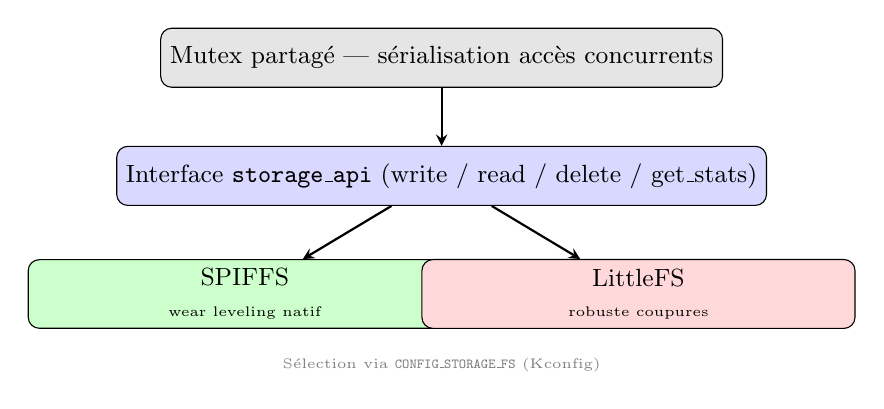
\begin{tikzpicture}[font=\small,
  box/.style={draw, rounded corners=4pt, minimum width=5.5cm,
              minimum height=0.75cm, align=center, fill=#1},
  arr/.style={->, thick, >=stealth}
]
  \node[box=gray!20] (mutex) at (0, 3.0)
        {Mutex partagé --- sérialisation accès concurrents};
  \node[box=blue!15] (api) at (0, 1.5)
        {Interface \texttt{storage\_api} (write / read / delete / get\_stats)};
  \node[box=green!20] (spiffs) at (-2.5, 0)
        {SPIFFS\\{\tiny wear leveling natif}};
  \node[box=red!15] (lfs) at (2.5, 0)
        {LittleFS\\{\tiny robuste coupures}};
  \node[font=\tiny, gray] (sel) at (0, -0.9)
        {Sélection via \texttt{CONFIG\_STORAGE\_FS} (Kconfig)};
  \draw[arr] (mutex) -- (api);
  \draw[arr] (api) -- (spiffs);
  \draw[arr] (api) -- (lfs);
\end{tikzpicture}%
}
\caption{Architecture du composant \texttt{storage\_api} --- abstraction SPIFFS/LittleFS avec mutex partagé}
\label{fig:storage_api}
\end{figure}

%------------------------------------------------------------
\subsection{Définition des partitions log/config/offline}
\label{subsec:storage_parts}
%------------------------------------------------------------

\begin{table}[H]
\centering
\renewcommand{\arraystretch}{1.6}
\caption{Schéma de partitionnement Flash du firmware \textit{GlobalFleet} --- \texttt{partitions.csv}}
\label{tab:partitions}
\small
\begin{tabular}{|p{2.8cm}|p{1.6cm}|p{1.6cm}|p{1.4cm}|p{3.5cm}|}
\hline
\rowcolor{gray!20}
\textbf{Partition} & \textbf{Type} & \textbf{Sous-type} & \textbf{Taille} & \textbf{Rôle} \\
\hline
\texttt{nvs}         & data & nvs    & 24\,Ko   & Config NVS + capabilities register \\
\hline
\texttt{otadata}     & data & ota    & 8\,Ko    & Métadonnées OTA Dual-Bank \\
\hline
\texttt{nvs\_factory}& data & nvs    & 16\,Ko   & Config usine factory (R/O) \\
\hline
\texttt{ota\_0}      & app  & ota\_0 & 1,5\,Mo  & Banque firmware A (active) \\
\hline
\texttt{ota\_1}      & app  & ota\_1 & 1,5\,Mo  & Banque firmware B (passive FOTA) \\
\hline
\texttt{logs}        & data & spiffs & 384\,Ko  & Ring buffer logs persistés \\
\hline
\texttt{offline}     & data & spiffs & 128\,Ko  & Trames GPS/CAN offline \\
\hline
\texttt{diag}        & data & nvs    & 32\,Ko   & Snapshots diagnostic post-mortem \\
\hline
\end{tabular}
\end{table}

\begin{figure}[H]
\centering
\resizebox{0.65\textwidth}{!}{%
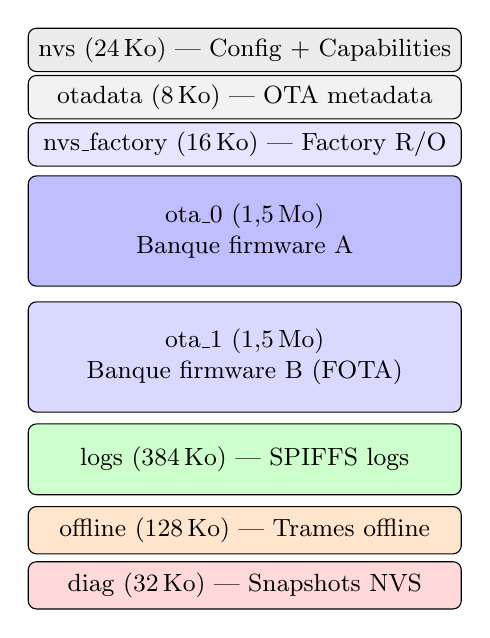
\begin{tikzpicture}[font=\small,
  part/.style 2 args={draw, rounded corners=3pt, minimum width=5.5cm,
               minimum height=#2, align=center, fill=#1}
]
  \node[part={gray!15}{0.5cm}]  at (0, 7.2)  {nvs (24\,Ko) --- Config + Capabilities};
  \node[part={gray!10}{0.4cm}]  at (0, 6.6)  {otadata (8\,Ko) --- OTA metadata};
  \node[part={blue!10}{0.5cm}]  at (0, 6.0)  {nvs\_factory (16\,Ko) --- Factory R/O};
  \node[part={blue!25}{1.4cm}]  at (0, 4.9)  {ota\_0 (1,5\,Mo)\\Banque firmware A};
  \node[part={blue!15}{1.4cm}]  at (0, 3.3)  {ota\_1 (1,5\,Mo)\\Banque firmware B (FOTA)};
  \node[part={green!20}{0.9cm}] at (0, 2.0)  {logs (384\,Ko) --- SPIFFS logs};
  \node[part={orange!20}{0.6cm}]at (0, 1.1)  {offline (128\,Ko) --- Trames offline};
  \node[part={red!15}{0.6cm}]   at (0, 0.4)  {diag (32\,Ko) --- Snapshots NVS};
\end{tikzpicture}%
}
\caption{Schéma de partitionnement Flash 16\,Mo du firmware \textit{GlobalFleet}}
\label{fig:partitions}
\end{figure}

%------------------------------------------------------------
\subsection{Gestion de l'endurance flash}
\label{subsec:storage_endur}
%------------------------------------------------------------

La Flash NOR de l'ESP32-P4 supporte typiquement 100\,000 cycles
d'effacement par secteur de 4\,Ko. Pour un appareil télématique
générant des logs en continu sur une durée de vie de plusieurs années,
sans stratégie de protection, cette limite pourrait être atteinte
prématurément sur les secteurs les plus sollicités. Trois mécanismes
complémentaires sont mis en place pour préserver l'endurance. Le ring
buffer RAM amortit les écritures : les entrées de log sont accumulées
en mémoire et purgées vers la Flash par lots de taille configurable
(\texttt{CONFIG\_LOG\_FLUSH\_BATCH\_SIZE}), réduisant la fréquence
d'effacement d'un facteur égal à la taille du lot. Les partitions
SPIFFS activent le mécanisme de nivellement d'usure
(\textit{wear leveling}) natif, répartissant les effacements sur
l'ensemble des secteurs disponibles plutôt que de concentrer l'usure
sur les secteurs les plus fréquemment écrits. La configuration field
n'est persistée que lors d'un appel explicite à \texttt{config\_apply()},
évitant les écritures fréquentes pour des changements incrémentaux
qui pourraient survenir à haute fréquence lors de mises à jour de
paramètres en temps réel.

%------------------------------------------------------------
\subsection{Ring buffer simple}
\label{subsec:ringbuf}
%------------------------------------------------------------

Le composant \texttt{ring\_buffer} est implémenté comme une structure
à deux indices (\texttt{head} et \texttt{tail}) sur un tableau statique
de taille \texttt{CONFIG\_RING\_BUF\_SIZE} définie à la compilation.
L'écriture incrémente \texttt{head} modulo la taille et écrase l'entrée
la plus ancienne si le buffer est plein (politique
\textit{overwrite-oldest}), garantissant que les entrées les plus
récentes sont toujours préservées, au détriment des entrées les plus
anciennes. Ce comportement est adapté au cas d'usage log où les
entrées récentes sont plus précieuses pour le diagnostic que les
entrées historiques. L'accès concurrent entre la tâche productrice
(module qui génère le log) et la tâche consommatrice
(\texttt{task\_storage} qui purge vers la Flash) est protégé par un
mutex récursif créé lors de l'initialisation du composant, garantissant
l'absence de corruption de l'état interne du ring buffer lors d'accès
simultanés.

%============================================================
\section{Implémentation du module Logger}
\label{sec:logger_impl}
%============================================================

%------------------------------------------------------------
\subsection{Niveaux de logs}
\label{subsec:loglevels}
%------------------------------------------------------------

Le module \texttt{logger} supporte quatre niveaux de sévérité
croissante, en cohérence avec les pratiques des systèmes embarqués
industriels. Le niveau \texttt{DEBUG} couvre les traces de développement
détaillées, activées uniquement en build de développement et exclues
du binaire de production via le symbole Kconfig
\texttt{CONFIG\_LOG\_MIN\_LEVEL}. Le niveau \texttt{INFO} documente
les événements nominaux du fonctionnement : démarrages de modules,
transitions FSM, connexions établies, envois réussis. Le niveau
\texttt{WARNING} signale les anomalies non critiques nécessitant
attention : activation du fallback config, compteur de santé en hausse,
approche du seuil de saturation du stockage. Le niveau \texttt{ERROR}
documente les défaillances traitées par la politique de récupération.
Le niveau minimal compilé est configurable via
\texttt{CONFIG\_LOG\_MIN\_LEVEL} dans \texttt{sdkconfig}, permettant
d'exclure les traces \texttt{DEBUG} du binaire de production sans
modifier une seule ligne du code source, ce qui est essentiel pour
maîtriser l'empreinte mémoire Flash du firmware en production.

%------------------------------------------------------------
\subsection{Logs structurés}
\label{subsec:logstruct}
%------------------------------------------------------------

Chaque entrée de log est sérialisée au format JSON compact sur une
seule ligne, facilitant le parsing automatisé côté serveur et
l'intégration avec les outils d'analyse de logs standards. Le format
retenu est le suivant :

\begin{verbatim}
{"ts":12345,"lvl":"W","mod":"config_manager","msg":"CRC invalid, fallback"}
\end{verbatim}

Les champs sont : \texttt{ts} (timestamp en millisecondes depuis le
boot, issu de \texttt{xTaskGetTickCount()}), \texttt{lvl} (niveau de
sévérité sur un caractère : E, W, I, D), \texttt{mod} (nom du module
émetteur, 16 caractères maximum), et \texttt{msg} (message libre,
128 caractères maximum). La taille fixe maximale de chaque entrée
(environ 170 octets) garantit que le dimensionnement du ring buffer
RAM est déterministe et calculable statiquement à la conception, sans
dépendance à la longueur variable des messages en production.

%------------------------------------------------------------
\subsection{Ring buffer de logs}
\label{subsec:logring}
%------------------------------------------------------------

Le module \texttt{logger} maintient un ring buffer RAM dédié,
instancié depuis le composant \texttt{ring\_buffer}, de
\texttt{CONFIG\_LOG\_RING\_SIZE} entrées (64 par défaut, configurable
jusqu'à 256 selon la mémoire disponible). Les entrées \texttt{DEBUG}
et \texttt{INFO} sont uniquement placées dans ce ring buffer, sans
émission sur UART en production, pour minimiser la charge de traitement.
Les entrées \texttt{WARNING} et \texttt{ERROR} sont également émises
immédiatement sur UART via \texttt{ESP\_LOGx()} pour les diagnostics
en temps réel lors des interventions terrain. La tâche
\texttt{task\_storage} consomme le ring buffer périodiquement selon
la période du timer de rotation et persiste les entrées dans la
partition \texttt{logs} via \texttt{storage\_api}, garantissant que
les logs survivent aux redémarrages et aux coupures d'alimentation.

%------------------------------------------------------------
\subsection{Rotation lorsque le buffer est plein}
\label{subsec:logrot}
%------------------------------------------------------------

Lorsque la partition \texttt{logs} atteint le seuil de remplissage
\texttt{CONFIG\_LOG\_ROTATION\_THRESHOLD} (80\,\% par défaut),
la rotation est déclenchée par la tâche \texttt{task\_storage}.
L'opération de rotation renomme le fichier courant \texttt{log.cur}
en \texttt{log.old} et crée un nouveau fichier \texttt{log.cur} vide,
puis publie l'événement \texttt{EVT\_STORAGE\_FULL} sur l'event bus
pour notification éventuelle au serveur de gestion de flotte via le
\texttt{comms\_manager}. L'ancien fichier \texttt{log.old} est
conservé jusqu'à la prochaine rotation, fournissant un historique
d'une période complète, soit environ 8 heures de logs \texttt{INFO}
au rythme d'une entrée par minute pour la variante Basic.

%------------------------------------------------------------
\subsection{Dump logs via UART/console}
\label{subsec:logdump}
%------------------------------------------------------------

Une commande de diagnostic \texttt{log dump [n]} est exposée sur le
port série via le composant \texttt{serial\_comm}, retournant les
\texttt{n} dernières entrées du ring buffer RAM au format JSON sur
UART. Cette commande est utile pour le débogage sur le terrain sans
accès à un serveur distant ou à l'infrastructure MQTT. Elle est
implémentée dans la tâche \texttt{task\_config} qui surveille les
commandes entrantes sur UART et les route vers les handlers appropriés.
En complément du dump RAM, la commande \texttt{log read [filename]}
permet de lire les entrées persistées sur la partition Flash \texttt{logs},
offrant un historique complet des événements depuis le dernier
démarrage ou depuis la dernière rotation.

%============================================================
\section{Implémentation du Power Manager}
\label{sec:power_impl}
%============================================================

%------------------------------------------------------------
\subsection{Règles RUN/SLEEP}
\label{subsec:power_rules}
%------------------------------------------------------------

Le composant \texttt{power\_manager} évalue périodiquement, toutes
les \texttt{cfg.power.eval\_period\_ms} millisecondes, un ensemble
de conditions pour décider d'une transition de mode énergétique.
La transition vers \texttt{SLEEP} est déclenchée si les trois
conditions suivantes sont simultanément vérifiées : absence de
mouvement détectée par l'accéléromètre (fourni par le composant
\texttt{sensors}) depuis plus de \texttt{T\_idle} secondes, absence
de connectivité réseau active signalée par le \texttt{comms\_manager},
et tension batterie supérieure au seuil de sécurité \texttt{V\_min}
lue via \texttt{hal\_gpio}. Le retour en \texttt{RUN} est déclenché
immédiatement dès que l'une des sources de réveil configurées dans
la partition \texttt{nvs\_field} est activée. Cette évaluation
multicritère garantit que le firmware n'entre en veille que lorsqu'il
est effectivement inactif, évitant d'interrompre une transmission
en cours ou une séquence de diagnostic active.

%------------------------------------------------------------
\subsection{Sources de réveil : timer et IO}
\label{subsec:power_wake}
%------------------------------------------------------------

Trois sources de réveil sont supportées et configurables via la
partition \texttt{nvs\_field}. Le timer périodique, géré par le
coprocesseur LP de l'ESP32-P4, réveille le système toutes les
\texttt{cfg.power.wake\_period\_s} secondes pour une transmission
de position minimale, garantissant la traçabilité du véhicule même
en stationnement prolongé. L'interruption GPIO sur le signal
d'allumage véhicule (\textit{ignition sense}), surveillée par le
composant \texttt{hal\_gpio}, réveille le système immédiatement lors
du démarrage du moteur, assurant la continuité du tracking dès la
mise en route. L'interruption de l'accéléromètre, dont le seuil de
mouvement est configurable via \texttt{cfg.power.accel\_threshold\_mg},
permet de détecter une manipulation ou un déplacement du véhicule
en stationnement. Les sources actives sont configurables
indépendamment, permettant d'ajuster finement le compromis entre
autonomie batterie et réactivité de détection selon le profil d'usage
de chaque véhicule.

%------------------------------------------------------------
\subsection{Réduction de l'activité système}
\label{subsec:power_reduce}
%------------------------------------------------------------

Avant d'entrer en mode \texttt{SLEEP}, le composant \texttt{power\_manager}
publie \texttt{EVT\_POWER\_SLEEP} sur l'event bus et attend que chaque
module abonné confirme son arrêt propre dans un délai
\texttt{cfg.power.shutdown\_timeout\_ms}. Cette synchronisation
garantit que toutes les écritures Flash en cours sont terminées via
\texttt{storage\_api}, que le buffer offline est vidé si de la
connectivité est disponible, et que les snapshots de diagnostic en
attente sont persistés en NVS via le composant \texttt{diagnostic}.
En cas de timeout d'un module lors de cette phase d'arrêt ordonné,
le module est forcément arrêté par le \texttt{power\_manager} et une
entrée \texttt{WARNING} est ajoutée au \texttt{logger} avec l'identifiant
du module défaillant, permettant l'identification a posteriori des
modules présentant des problèmes d'arrêt propre.

%------------------------------------------------------------
\subsection{Démonstration RUN$\rightarrow$SLEEP et SLEEP$\rightarrow$RUN}
\label{subsec:power_demo}
%------------------------------------------------------------

La démonstration de la transition énergétique est réalisée en
déclenchant artificiellement le passage en veille par simulation
d'inactivité prolongée (injection de l'événement via le canal
\texttt{serial\_comm}) et en observant les logs UART. Les métriques
attendues selon les critères d'acceptation du chapitre~V sont un temps
de transition RUN$\rightarrow$SLEEP inférieur à
\texttt{cfg.power.shutdown\_timeout\_ms} (200\,ms par défaut), une
consommation en mode \texttt{SLEEP} inférieure à 5\,mA pour toutes
les variantes, et un temps de transition SLEEP$\rightarrow$RUN
inférieur à 500\,ms pour une reprise complète du fonctionnement nominal.

% [ESPACE RÉSULTATS --- insérer logs UART de transition et
%  mesures de consommation avant/après en mA]

%============================================================
\section{Implémentation du Diagnostic}
\label{sec:diag_impl}
%============================================================

%------------------------------------------------------------
\subsection{Reset reason}
\label{subsec:diag_reset}
%------------------------------------------------------------

La raison du dernier redémarrage est lue via l'API ESP-IDF
\texttt{esp\_reset\_reason()} au démarrage, avant toute autre
initialisation, et persistée dans la partition \texttt{diag} avec
un horodatage. Les valeurs possibles couvrent l'ensemble des causes
de redémarrage de l'ESP32-P4 : reset power-on (\texttt{ESP\_RST\_POWERON}),
reset watchdog matériel (\texttt{ESP\_RST\_WDT}), reset logiciel
(\texttt{ESP\_RST\_SW}), reset panique ou assertion échouée
(\texttt{ESP\_RST\_PANIC}), et reset consécutif à une mise à jour
OTA (\texttt{ESP\_RST\_DEEPSLEEP}). Cette information est exposée
dans le status report périodique envoyé au serveur et enrichit les
snapshots de diagnostic en cas de transition vers l'état \texttt{FAULT},
permettant de distinguer les redémarrages normaux (post-OTA) des
redémarrages anormaux (watchdog, panique) dans les analyses de flotte.

%------------------------------------------------------------
\subsection{Uptime}
\label{subsec:diag_uptime}
%------------------------------------------------------------

Le temps de fonctionnement cumulé (\textit{uptime}) est calculé à
partir du tick FreeRTOS via \texttt{xTaskGetTickCount()}, converti
en secondes selon la fréquence de tick configurée (1000\,Hz). Deux
valeurs distinctes sont maintenues par le composant \texttt{diagnostic}.
L'\texttt{uptime\_boot} mesure le temps écoulé depuis le dernier
redémarrage, utile pour identifier des redémarrages fréquents
indiquant une instabilité. L'\texttt{uptime\_total} cumule le temps
de fonctionnement sur l'ensemble de la vie de l'appareil, persisté
en NVS à chaque snapshot, permettant de calculer des métriques de
disponibilité à l'échelle de la flotte. La dérivée de
\texttt{uptime\_total} entre deux status reports consécutifs permet
au serveur de détecter une fréquence de redémarrage anormale sans
accès physique à l'appareil.

%------------------------------------------------------------
\subsection{Snapshots système}
\label{subsec:diag_snap}
%------------------------------------------------------------

Un snapshot est une structure C sérialisée au format JSON, capturant
l'état complet du système à un instant donné. Elle contient : la
reset reason et l'uptime, l'état (\texttt{IDLE}/\texttt{RUNNING}/
\texttt{DEGRADED}/\texttt{FAULT}) et le health counter de chaque
module actif, le heap libre et le watermark de stack par tâche
FreeRTOS (via \texttt{uxTaskGetStackHighWaterMark()}), les statistiques
réseau (\texttt{comms\_manager}), et les 10 dernières entrées du
ring buffer de logs. Les snapshots sont déclenchés automatiquement
lors de la transition vers l'état \texttt{FAULT} (invoqué par le
\texttt{fault\_manager}), ou à la demande via la commande
\texttt{diag snapshot} sur le canal \texttt{serial\_comm}. Ils sont
persistés dans la partition NVS \texttt{diag} et transmis au serveur
lors du rétablissement de la connectivité, permettant un diagnostic
post-mortem précis des incidents survenus hors connectivité.

%------------------------------------------------------------
\subsection{État des modules}
\label{subsec:diag_mods}
%------------------------------------------------------------

Le composant \texttt{diagnostic} maintient un tableau d'état pour
chaque module enregistré via \texttt{diag\_register\_module(id, name)}.
L'état est mis à jour par les modules eux-mêmes via l'API
\texttt{diag\_set\_module\_state(id, state)}, permettant au composant
\texttt{diagnostic} de refléter fidèlement l'état réel de chaque
composant sans nécessiter d'interrogation active. Ce tableau est
inclus dans chaque snapshot et dans le status report périodique,
sérialisé au format JSON dans le champ \texttt{modules\_state}. Le
serveur de gestion de flotte peut ainsi détecter en temps réel les
modules dégradés (\texttt{DEGRADED}) ou en faute (\texttt{FAULT})
dans l'ensemble de la flotte, déclencher des interventions préventives
avant que les dégradations n'affectent la qualité de service, et
identifier les composants instables corrélés à certains modèles de
matériel ou à certaines configurations terrain.

%------------------------------------------------------------
\subsection{Status report structuré}
\label{subsec:diag_report}
%------------------------------------------------------------

Le status report est un message JSON périodique publié via le
\texttt{comms\_manager} sur le topic MQTT
\texttt{sat/<device\_id>/diagnostic}. Il contient : l'identifiant
du dispositif, le profil de capacités actif (valeur du registre
32~bits), l'uptime, la version firmware (tag Git compilé en dur via
\texttt{\_\_DATE\_\_} et \texttt{IDF\_VER}), l'état de chaque module,
le heap libre, la consommation estimée selon le mode courant, et
l'indicateur \texttt{config\_fallback\_active}. La période de
publication est configurée via \texttt{cfg.comms.diag\_report\_interval\_s}
(300~secondes par défaut, ajustable à distance). Ce report constitue
le principal canal de monitoring de la flotte, permettant au serveur
de détecter proactivement les appareils nécessitant une intervention
sans attendre leur signalement.

%============================================================
\section{Modularité et intégration}
\label{sec:modularite}
%============================================================

%------------------------------------------------------------
\subsection{HAL v1}
\label{subsec:hal_v1}
%------------------------------------------------------------

La HAL v1 implémente les interfaces pour les deux drivers physiques
fournis dans le composant \texttt{hal\_driver} : \texttt{hal\_gpio}
pour la gestion des entrées/sorties numériques (signal d'allumage,
LED de statut, contrôle des alimentations périphériques) et
\texttt{hal\_uart} pour la communication série asynchrone (réception
NMEA du module GNSS, communication locale \texttt{serial\_comm}).
Les stubs de test pour le composant \texttt{gps} et les entrées GPIO
sont fournis dans \texttt{test\_host/} sous la forme de modules C
injectables via des pointeurs de fonctions. Chaque driver implémente
les quatre primitives standardisées \texttt{drv\_init()},
\texttt{drv\_read()}, \texttt{drv\_write()} et \texttt{drv\_deinit()}
définies dans les fichiers \texttt{hal\_gpio.h} et \texttt{hal\_uart.h},
exposant une interface stable et substituable par un mock dans les
environnements de test hors-cible.

%------------------------------------------------------------
\subsection{Guide d'ajout d'un driver}
\label{subsec:hal_guide}
%------------------------------------------------------------

L'intégration d'un nouveau driver HAL dans le projet \textit{GlobalFleet}
suit quatre étapes documentées et reproductibles. \textbf{Étape~1} :
créer le fichier d'interface \texttt{hal\_xxx.h} dans
\texttt{components/hal\_driver/include/} déclarant la structure de
configuration du driver et les quatre primitives standardisées.
\textbf{Étape~2} : implémenter le driver dans
\texttt{components/hal\_driver/src/hal\_xxx.c} en s'appuyant
uniquement sur les primitives ESP-IDF, sans référencer aucun service
applicatif. \textbf{Étape~3} : enregistrer le bit de capacité
correspondant dans \texttt{capabilities.h} et déclarer la fonctionnalité
dans le tableau des variantes du \texttt{config\_manager}. \textbf{Étape~4} :
créer le stub de test dans \texttt{test\_host/} retournant des données
simulées configurables par les scripts Python
(\texttt{test\_subscription.py}, \texttt{mqtt\_test.py}), et ajouter
le cas de test Unity correspondant pour valider l'interface.

%------------------------------------------------------------
\subsection{Stubs GNSS et IO}
\label{subsec:hal_stubs_impl}
%------------------------------------------------------------

Les stubs GNSS et IO présents dans \texttt{test\_host/} permettent
de valider les services applicatifs sur machine de développement sans
aucun matériel physique. Le stub GNSS, référencé dans
\texttt{test\_subscription.c}, retourne des trames NMEA
pré-enregistrées ou générées synthétiquement depuis un fichier de
replay, permettant de simuler des scénarios de navigation réels
(acquisition de fix, perte de signal, passage en zone à couverture
partielle). Le stub IO simule les transitions du signal d'allumage
véhicule et les événements de l'accéléromètre via des commandes Python
injectées dans la file d'événements de l'\texttt{event\_bus} par le
script \texttt{test\_subscription.py}. Ces stubs sont la pierre
angulaire de la stratégie de tests hors-cible, permettant d'exécuter
les scénarios de test de robustesse (transitions FSM, déclenchement
du watchdog, saturation du stockage) en quelques secondes sur machine
de développement, sans nécessiter de matériel physique ni de
connectivité.

%------------------------------------------------------------
\subsection{Sélecteur de protocole runtime}
\label{subsec:proto_sel}
%------------------------------------------------------------

Le sélecteur de protocole est implémenté dans
\texttt{components/comms\_provider/src/comms\_provider.c} comme une
table de pointeurs de fonctions (\texttt{comms\_provider\_ops\_t})
initialisée au démarrage selon la valeur de \texttt{cfg.comms.protocol}
lue depuis \texttt{config\_manager}. Trois entrées sont disponibles
dans la table : l'implémentation MQTT/TLS~1.3 (recommandée pour Pro
et Ultra-Pro), l'implémentation TCP brut avec TLS optionnel, et
l'implémentation UDP sans garantie de livraison pour les trames haute
fréquence. L'appel à \texttt{comms\_publish(topic, payload, qos)}
par un module producteur est strictement indépendant du protocole
actif : le \texttt{comms\_manager} route l'appel vers l'implémentation
instanciée sans que le module producteur n'ait connaissance du protocole
sous-jacent. Le changement de protocole via \texttt{config\_apply()}
provoque la réinstanciation de la table lors de la prochaine connexion,
sans redémarrage du système.

%------------------------------------------------------------
\subsection{Intégration avec l'axe configuration/diagnostic}
\label{subsec:integ_cfg_diag}
%------------------------------------------------------------

La chaîne d'intégration \texttt{config\_manager}$\leftrightarrow$\texttt{diagnostic}
fonctionne entièrement via l'\texttt{event\_bus}, sans couplage
direct entre les deux composants. Toute modification de configuration
validée via \texttt{config\_apply()} publie \texttt{EVT\_CONFIG\_CHANGED}.
Le composant \texttt{diagnostic}, abonné à cet événement, enregistre
automatiquement la modification dans le snapshot courant avec
horodatage et valeurs avant/après, constituant un journal d'audit
de la configuration accessible au serveur. Si la modification concerne
un paramètre critique --- protocole de communication, politique de veille,
seuils de détection --- le \texttt{diagnostic} déclenche immédiatement
un nouveau status report vers le serveur pour confirmer la prise en
compte de la configuration, sans attendre la prochaine période de
rapport périodique. Ce mécanisme garantit que le serveur est toujours
informé des changements de configuration en moins d'un cycle de
reporting.

%------------------------------------------------------------
\subsection{Canal réel USB ou BLE pour config/diag}
\label{subsec:canal_reel}
%------------------------------------------------------------

En complément du canal MQTT, un canal de configuration locale est
exposé via le port USB-Serial natif de l'ESP32-P4, géré par le
composant \texttt{serial\_comm} appuyé sur le driver \texttt{hal\_uart}.
Ce canal accepte des commandes textuelles au format JSON pour lire
et modifier la configuration field (\texttt{config get <key>},
\texttt{config set <key> <value>}), déclencher un dump de logs
(\texttt{log dump <n>}), ou forcer un snapshot de diagnostic
(\texttt{diag snapshot}). En variante Ultra-Pro (bit~3 du registre
de capacités), ce même jeu de commandes est exposé via BLE~5.0,
permettant la configuration sans câble via une application mobile.
Les deux canaux partagent le même parseur de commandes JSON, défini
dans un module commun, garantissant la cohérence des opérations et
la parité fonctionnelle entre les deux canaux.

%============================================================
\section{Gestion des incidents}
\label{sec:incidents}
%============================================================

%------------------------------------------------------------
\subsection{Policies FAULT}
\label{subsec:fault_pol}
%------------------------------------------------------------

La politique de traitement des fautes est implémentée dans le composant
\texttt{fault\_manager} comme une table de dispatch associant chaque
niveau de sévérité à une fonction de traitement. À la réception d'un
événement de faute (\texttt{EVT\_WDT\_TIMEOUT},
\texttt{EVT\_FAULT\_DETECTED}, \texttt{EVT\_FAULT\_CRITICAL}), le
\texttt{fault\_manager} consulte la table, exécute la fonction de
traitement correspondante, et enregistre la faute dans le catalogue
interne. Les actions sont exécutées séquentiellement dans l'ordre
croissant de sévérité : journalisation via \texttt{logger}, puis
redémarrage du module fautif via son interface \texttt{module\_stop()}
/ \texttt{module\_start()}, puis redémarrage système complet en
publiant \texttt{EVT\_FAULT\_CRITICAL} depuis lui-même, puis activation
du mode safe. Chaque action est conditionnée par une vérification
préalable : l'escalade vers le niveau supérieur n'intervient que si
l'action du niveau courant a échoué ou si le seuil d'occurrences
est dépassé.

%------------------------------------------------------------
\subsection{Backoff}
\label{subsec:backoff}
%------------------------------------------------------------

Le backoff exponentiel est appliqué par le \texttt{fault\_manager}
aux redémarrages de modules de niveau ERROR. La séquence de délais
d'attente avant chaque tentative de redémarrage est : 1\,s, 2\,s,
4\,s, 8\,s, plafonnée à 16\,s pour les tentatives suivantes. Pendant
le délai de backoff, le module est dans l'état \texttt{FAULT} et
ses abonnements sur l'\texttt{event\_bus} sont suspendus pour éviter
l'accumulation d'événements non traités dans la file. Le compteur
de tentatives est réinitialisé si le module fonctionne nominalement
pendant plus de \texttt{cfg.error.recovery\_window\_s} secondes
consécutives après un redémarrage réussi, évitant qu'un module
historiquement fragile soit définitivement bloqué par un compteur
élevé suite à un incident passager et isolé. Cette politique de
réinitialisation du compteur garantit que le comportement du firmware
est prédictible même après des incidents répétés séparés dans le
temps.

%------------------------------------------------------------
\subsection{Mode safe}
\label{subsec:safemode}
%------------------------------------------------------------

Le mode safe minimal est activé par le \texttt{fault\_manager} lorsque
la politique FATAL est déclenchée, soit par le mécanisme anti-boucle
après trois redémarrages en moins de 60~secondes. Dans ce mode,
seuls trois composants restent actifs : le \texttt{comms\_manager}
en mode connexion minimale (sans MQTT, uniquement TCP brut) pour
permettre la transmission du rapport de diagnostic, le composant
\texttt{diagnostic} pour la génération et la persistance du snapshot
post-mortem complet, et le \texttt{config\_manager} en lecture seule
pour permettre une intervention de reconfiguration distante. Tous
les autres composants sont arrêtés proprement via leur interface
\texttt{module\_stop()}. Un flag \texttt{safe\_mode\_active} est
persisté en NVS par le \texttt{config\_manager} pour signalement
au redémarrage suivant, permettant au firmware de démarrer
directement en mode diagnostic restreint sans tenter un démarrage
nominal qui échouerait à nouveau.

%------------------------------------------------------------
\subsection{Reprise après reboot}
\label{subsec:reboot_resume}
%------------------------------------------------------------

Au démarrage, le \texttt{config\_manager} vérifie la présence du
flag \texttt{safe\_mode\_active} dans la partition NVS lors de la
troisième étape de la séquence de boot. Si le flag est présent, le
firmware démarre en mode diagnostic restreint : seuls les trois
composants du mode safe sont initialisés et démarrés, aucune tâche
applicative n'est créée, et un message de diagnostic est immédiatement
envoyé au serveur via \texttt{comms\_manager} indiquant l'état dégradé
et la cause de la faute originelle. Ce mode attend une commande
explicite de remise en service (\texttt{RESET\_SAFE\_MODE}) envoyée
par le serveur sur le topic MQTT \texttt{sat/<device\_id>/cmd/system}
ou via le canal \texttt{serial\_comm} local, avant de réinitialiser
le flag et d'initier un redémarrage complet vers le fonctionnement
normal. Ce mécanisme garantit que le retour à la normale est une
décision délibérée de l'opérateur, évitant une boucle de redémarrages
automatiques qui épuiserait la batterie et masquerait la cause racine
du problème.

%------------------------------------------------------------
\subsection{Protection contre les boucles d'erreurs}
\label{subsec:antiloop}
%------------------------------------------------------------

Le mécanisme anti-boucle, implémenté dans le \texttt{fault\_manager},
surveille le nombre de transitions vers l'état \texttt{FAULT} dans
une fenêtre glissante de 60~secondes. Il est implémenté comme un
compteur entier incrémenté à chaque transition FAULT et décrémenté
périodiquement par le timer anti-boucle selon la période
\texttt{cfg.error.reboot\_window\_s}. Le compteur et sa fenêtre
temporelle sont persistés en NVS pour résister aux coupures
d'alimentation : un appareil qui redémarre en boucle et perd
l'alimentation à chaque redémarrage ne perd pas le contexte de sa
boucle. Au-delà du seuil \texttt{cfg.error.reboot\_max\_count}
(trois par défaut), toute nouvelle faute est directement reclassifiée
\texttt{FATAL} et le mode safe est activé sans nouvelle tentative
de récupération. Les paramètres de seuil et de fenêtre sont
configurables via la partition \texttt{nvs\_field}, permettant
d'ajuster la politique d'anti-boucle selon le profil de criticité
de chaque déploiement.

%============================================================
\section{Conclusion}
\label{sec:conclu_ch4}
%============================================================
En résumé, ce chapitre a détaillé l'implémentation du firmware générique \textit{GlobalFleet} sous ESP-IDF~v5.3 pour l'ESP32-P4. Reposant sur une architecture FreeRTOS modulaire à neuf tâches et un bus \textit{Publish-Subscribe}, le système a été rigoureusement conçu selon une approche défensive. 

L'intégration de 23 composants indépendants via une interface standardisée (\texttt{module\_interface\_t}), couplée à un dispositif de récupération à quatre niveaux (watchdog, backoff exponentiel, anti-boucle et mode \textit{safe}), garantit une fiabilité et une maintenabilité optimales pour les déploiements industriels. La validation quantitative de ces mécanismes de robustesse fera l'objet du chapitre~V.